% Publication-Grade Causal DAG: Confounder (Backdoor Path)
% Adheres to Pearl (2009) and Cinelli, Forney, and Pearl (2022)
% Compile with pdflatex or lualatex

\documentclass[tikz,border=10pt]{standalone}
\usepackage{tikz}
\usetikzlibrary{arrows.meta,positioning,shapes.geometric}

\begin{document}
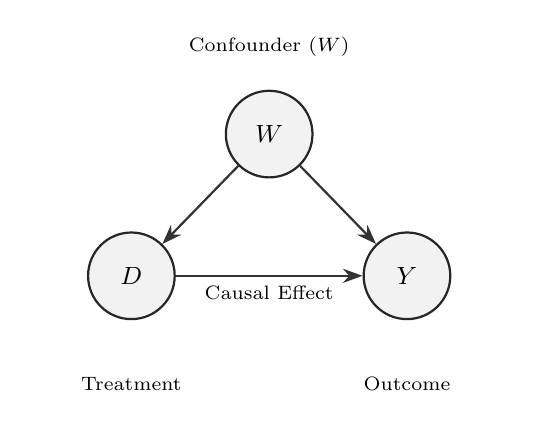
\begin{tikzpicture}[
    node distance=2.2cm and 2.5cm,
    every node/.style={font=\sffamily\small},
    observed/.style={circle, draw=black!85, fill=black!5, thick, minimum size=1.1cm},
    unobserved/.style={circle, draw=black!75, dashed, fill=black!2, thick, minimum size=1.1cm},
    edge/.style={->, >={Stealth[length=2.5mm, width=1.8mm]}, thick, draw=black!80},
    bi_edge/.style={<->, >={Stealth[length=2.5mm, width=1.8mm]}, thick, dashed, draw=black!70}
]

    % Nodes
    \node[observed] (X) at (0, 0) {$D$};
    \node[observed] (Y) at (3.5, 0) {$Y$};
    \node[observed] (W) at (1.75, 1.8) {$W$};

    % Edges
    \draw[edge] (X) -- node[below, font=\scriptsize] {Causal Effect} (Y);
    \draw[edge] (W) -- (X);
    \draw[edge] (W) -- (Y);

    % Legend or annotations
    \node[below=0.6cm of X, text width=2.4cm, align=center, font=\scriptsize] {Treatment};
    \node[below=0.6cm of Y, text width=2.4cm, align=center, font=\scriptsize] {Outcome};
    \node[above=0.3cm of W, text width=3.0cm, align=center, font=\scriptsize] {Confounder ($W$)};

\end{tikzpicture}
\end{document}
